\begin{figure}[h!]
\usetikzlibrary {circuits.logic.US}
\tikzset{
    grow'=down,
    level distance=42pt,
    % sibling distance=24pt,
    % sibling distance=8mm/#1,
    level/.style={sibling distance=3pt+44pt/(#1*#1*0.75)},
    edge from parent/.append style={
        draw,
        %thick,
        edge from parent path={
        (\tikzparentnode.west) |- ($(\tikzparentnode.west)!0.5!(\tikzchildnode.east)$) -| (\tikzchildnode.east)
        },
    },
    every node/.append style={
        anchor=center,
        rotate=90,
        draw=black,
        fill=white,
        thick,
        font=\footnotesize\bfseries,
        text centered,
        inner sep=0pt
    },
    var/.style={
        shape=circle,
        minimum height=16pt,
    },
    and/.style={
    and gate US,
    },
  not/.style={
    not gate US,
  },  
  or/.style={
    or gate US,
  },
  vot/.style={
    or gate US,
  }
}
  \centering
  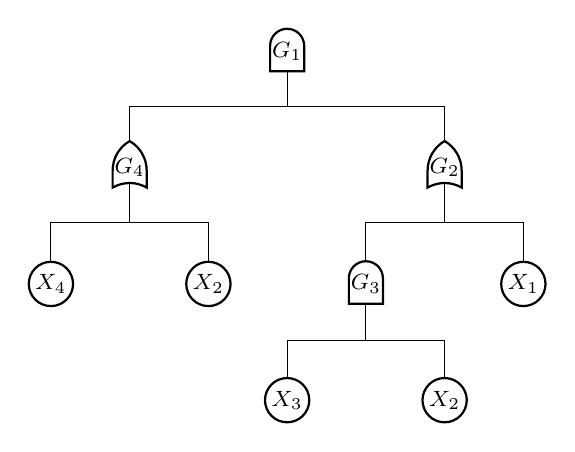
\begin{tikzpicture}[
    circuit logic US,
    tiny circuit symbols,
    level 1/.style={sibling distance=40mm},
    level 2/.style={sibling distance=20mm},
    level 3/.style={sibling distance=20mm}
    ]

    \node[and]{\rotatebox{-90}{$G_1$}}
    child { node[or] {\rotatebox{-90}{$G_2$}}
      child { node[var] {\rotatebox{-90}{$X_1$}} }
      child { node[and] {\rotatebox{-90}{$G_3$}}
        child { node[var] {\rotatebox{-90}{$X_2$}} }
        child { node[var] {\rotatebox{-90}{$X_3$}} }
      }
    }
    child { node[or] {\rotatebox{-90}{$G_4$}}
      child { node[var] {\rotatebox{-90}{$X_2$}} }
      child { node[var] {\rotatebox{-90}{$X_4$}} }
    };
  \end{tikzpicture}
  \caption{Sample fault tree for MOCUS demonstration.}
  \label{fig:sample_mocus_ft}
\end{figure}
